%% question-8.tex
%%

%% ==============================
\subsection{Modélisation du concept de Type}
\label{sec:question8}
%% ==============================

Le concept de \emph{Type} est modélisé de la manière présentée à la figure \ref{fig:type}. La classe \emph{Type} est parent de plusieurs classes présentes dans ce diagramme \emph{Enumération}, \emph{TypePrimitif},\emph{Tableau}. 

On peut remarquer que le type \emph{void} n'est pas considéré comme un type primitif et est donc directement relié à la classe \emph{Type}. 

\begin{figure}
	\centering
	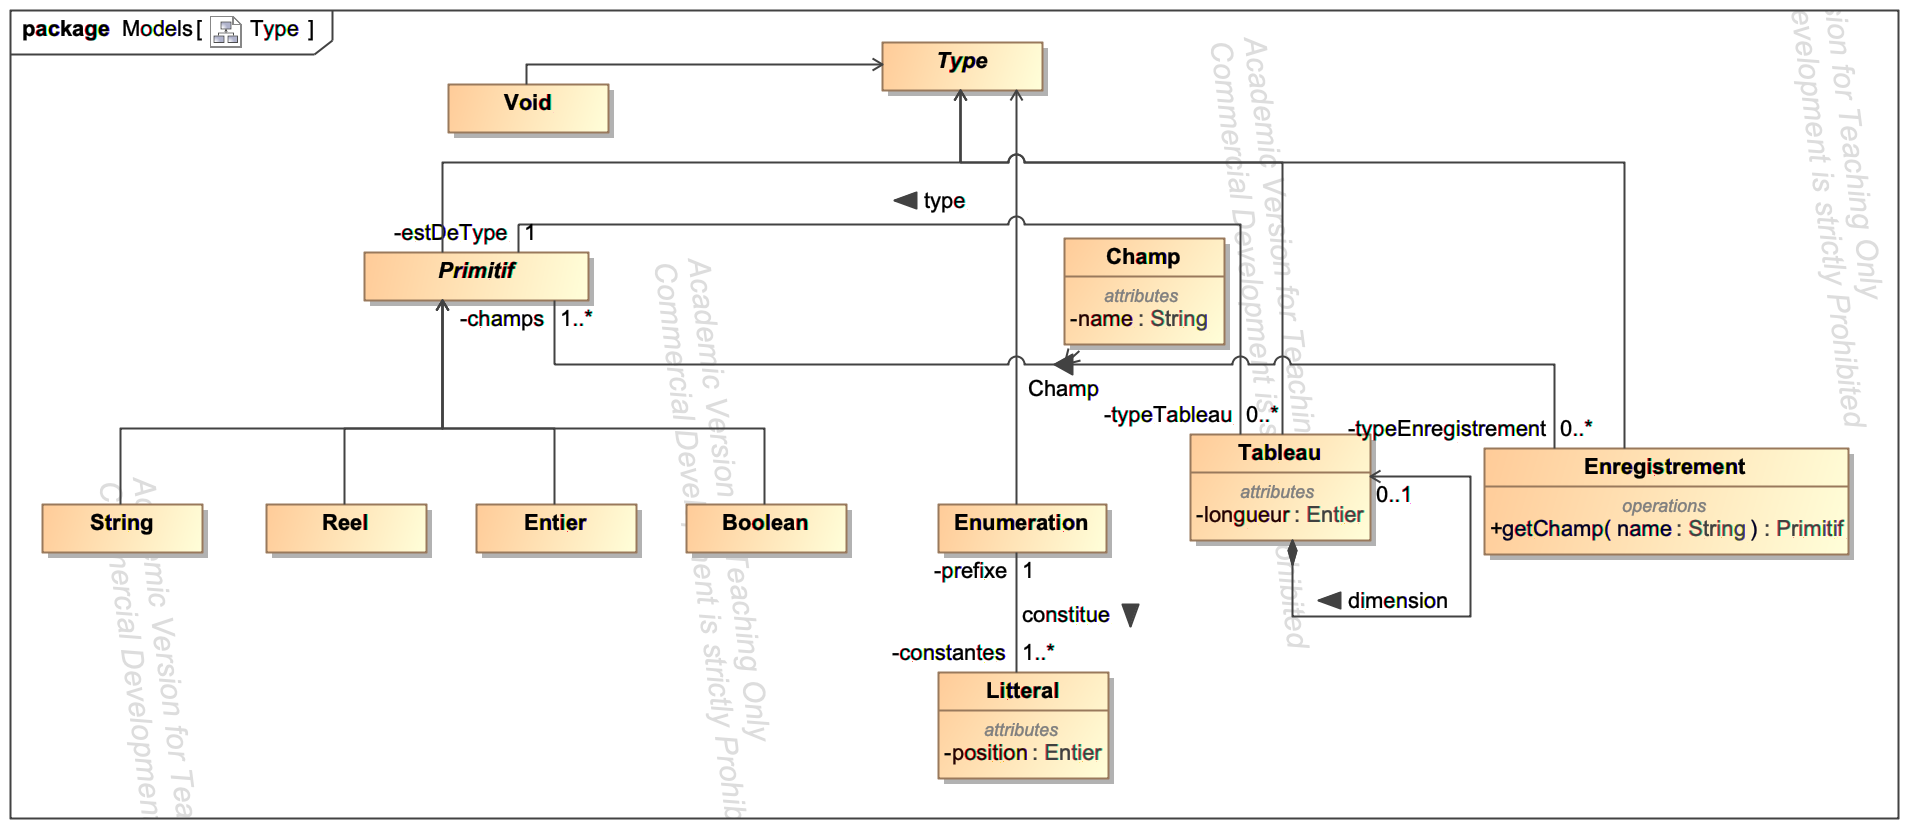
\includegraphics[width=500pt]{assets/class__Type}
	\caption{Diagramme de classe d'un type}
	\label{fig:type}
\end{figure}
